\section{Systematic uncertainties}\label{sec:WBoson_Systematics}

This section presents the different sources and the procedure employed to determine the systematic uncertainties in the measurement of the \W boson production in \pPb.

%%------------------------------------------------------------%%
\subsection{Luminosity}

The integrated luminosity of the 2016 \pPb data sample processed is $173.4 \pm 5\%$~\nbinv as presented in \sect{sec:WBoson_Samples_Data}. Since the integrated luminosity cancels in asymmetries, it only affects the measurement of the \WToMuNu differential cross sections. In this case, the systematic uncertainty is taken as a global uncertainty of 5$\%$ and the bin-to-bin correlation is +100$\%$.

%%------------------------------------------------------------%%
\subsection{Muon efficiency}

\subsubsection{MC statistics}

A systematic uncertainty is assigned to account for the limited statistics in the MC samples used to compute the muon efficiency. The MC statistical uncertainty of the muon efficiencies is computed using Bayesian statistics as explained in \sect{sec:WBoson_Efficiency} and then propagated to all the observables. The uncertainty is considered to be fully uncorrelated.

\subsubsection{Theory model}

The NLO model used to generate the MC samples can impact the measurement of the muon efficiencies. The main sources of theory uncertainties include the choice of the nuclear parton distribution function (EPPS16+CT14), renormalization scale, factorization scale and $\alpha_{s}$. The theory uncertainties are assumed to be correlated in both charge and $\eta_{CM}$.

Since the PDFs are not calculable from first principles but are determined experimentally, the inclusion of any PDF introduces an additional systematic error. Therefore, it is important to determine the impact of a change of PDF on the muon efficiencies. The procedure to derive the theory uncertainties of the PDF variations consist of reweighing the simulation using the weights produced by \POWHEG after applying each PDF set. The PDF sets are accessed through the LHAPDF6~\cite{LHAPDF6} framework and consist of 56 CT14 PDFs, 40 EPPS16 nuclear corrections and 2 CT14 $\alpha_{s}$ variations. Once the MC samples are reweighed with each PDF set, the efficiencies are recomputed and used to recalculate all the observables.

The nPDF uncertainty is determined by combining the EPPS16+CT14 variations of the observables using the Hessian approach as recommended by the EPPS16 authors (see Eq.~29 of Ref.~\cite{EPS09}). The EPPS16+CT14 sets corresponds to 90$\%$ confidence interval (CL) variations, so the uncertainties are scaled to 68$\%$.

Furthermore, the $\alpha_{s}$ uncertainty is determined by using the CT14 PDFs associated to the $\alpha_{s}\left(m_{Z}^{2}\right)$ values: 0.1170 and 0.1190. The variations on the observables are combined following the prescription recommended in the PDF4LHC15~\cite{PDF4LHC}, which basically corresponds to taking the average per bin of the two variations. The uncertainties are converted to 68$\%$ CL after rescaling them by $0.0015/0.0010$ as described in PDF4LHC15~\cite{PDF4LHC}.

And finally, the uncertainty due to the renormalization ($\mu_{R}$) and factorization ($\mu_{F}$) scales, is computed by varying the two scales in \POWHEG using the following combinations:
\begin{equation*}
(\mu_{R} , \mu_{F}) = [\ (0.5 , 0.5)\ ,\ (1.0 , 0.5)\ ,\ (0.5 , 1.0)\ ,\ (1.0 , 2.0)\ ,\ (2.0 , 1.0)\ ,\ (2.0 , 2.0)\ ]
\end{equation*}

The MC samples are reweighed event by event using the \POWHEG weights produced with each set of scales, then the efficiencies are recomputed and the observables are recalculated for each varied efficiency. The variations on the observables are combined by taking the envelope (i.e. the maximum variation in each $\eta_{CM}$ bin). The uncertainties are considered 68$\%$ CL.


\subsubsection{Tag-and-Probe correction}

The main source of systematic uncertainty in the measurement of the muon efficiency arises from the application of the TnP scale factors used to correct the truth efficiency. As mentioned in \sect{sec:WBoson_Efficiency_CorrectedEfficiency}, the statitstical and systematic uncertainties of the TnP correction is composed by the different components that enters the muon efficiency: trigger, identification, isolation, reconstruction, event activity and pileup.

Since \W boson asymmetries in muon pseudorapidity and charge are measured, it is crucial to consider the correlation between the different TnP uncertainties as a function of muon $\eta_{CM}$ and charge. The statistical TnP variations are considered correlated only within the $\eta_{LAB}$ bins (see \cite{Muon_TnP_pPb}) in which they were derived ($\eta_{LAB}$ bin in the case of trigger, $|\eta_{LAB}|$ bin in the case of identification and isolation), while no correlation is assumed with respect to the muon charge. The systematic TnP variations are expected to be fully correlated as a function of muon charge and uncorrelated between the different $\eta_{CM}$. The correlations of each source of TnP uncertainty are listed in \tab{tab:systcorr}.

\begin{table}[!htb]
 \begin{center}
 \begin{tabular}{l|c|c}
 \hline
 Source of uncertainty & correlation in muon $\eta$ & correlation in muon charge \\
 \hline
 Trigger, stat. & yes per $\eta$ range & no \\
 ID, stat. & yes per $|\eta|$ range & no \\
 Iso, stat. & yes per $|\eta|$ range & no \\
 Trigger, syst. & no & yes \\
 ID, syst. & no & yes \\
 Iso, syst. & no & yes \\
 ID, syst. binned & no & yes \\
 Iso, syst. binned & no & yes \\
 HF$+$PU & no & yes \\
 STA & no & yes \\
 \hline
 \end{tabular}
 \end{center}
 \caption{Summary of the correlations per source of tag and probe uncertainty, as a function of muon pseudorapidity (in the laboratory frame) and charge. When a correlation per $\eta$ or $|\eta|$ range is mentioned, the different ranges are uncorrelated between them.}
 \label{tab:systcorr}
\end{table}

To compute the uncertainties, the muon charge asymmetry and the forward-backward ratios are recalculated for each efficiency derived by varying the TnP scale factors. The TnP uncertainties are then determined by taking the difference between the value obtained with the varied TnP SF and its nominal value, combining the uncertainties as explained in \sect{sec:WBoson_Efficiency_CorrectedEfficiency}. If the TnP source is correlated in muon charge or pseudorapidity, the corresponding \W boson yields are varied at the same time. Moreover, for the $\W^{\pm}$ cross sections, the statistical and systematic TnP uncertainties are calculated by propagating the uncertainties on the corrected muon efficiency due to the TnP variations.

%%------------------------------------------------------------%%
\subsection{Choice of binning}


Since the \W signal distribution is parametrised using a binned MC template with a bin width of 2~\GeVc, the uncertainty on the signal template is determined by decreasing the bin width to 1~\GeVc. The systematic uncertainty is assigned for each $\eta_{CM}$ bin by taking the maximum difference between the nominal and the varied observables. The correlations bin-to-bin and between the positively and negatively charged muons is taken to be 100~$\%$.


%%------------------------------------------------------------%%
\subsection{QCD background}

The systematic uncertainty in the QCD background originates from the uncertainty in the modeling of the multi-jet MET distribution in the signal region. The nominal procedure consist on fixing the parameters of the modified Rayleigh distribution from the fits extrapolated from data as explained in Sec.~\ref{sec:WBoson_SignalExtraction_QCDBackground}. In order to estimate the uncertainty of the mismodeling of the QCD shape, both the parameters and the functional form are varied as explained in the following subsections.

\subsubsection{QCD model parameters}

The first source of systematic uncertainty reflects the possible mismodelling of the QCD shape due to the $\eta_{CM}$ dependence of the QCD parameters. In order to check this, the parameters of the nominal QCD model are set free but constrained to the weighted RMS and mean value of the extrapolated results extracted in each $\eta_{CM}$ bin. The values used to constrain the $\sigma_{0}$,  $\sigma_{1}$ and  $\sigma_{2}$ parameters are shown in \tab{tab:QCDContrainPar}. The average over $\eta_{CM}$ bins of the difference between the final observables derived from the constrained fits and the nominal results is taken as the systematic error. This source of uncertainty is taken to be fully uncorrelated.

\begin{table}[!h]
  \begin{center}
  \begin{tabular}{|c|c|c|}\hline
  Parameter & $QCD \to \mu^{-}$ & $QCD \to \mu^{+}$ \\\hline
  $\sigma_{0}$ & 14.49$\pm$0.95 & 14.78$\pm$0.52 \\\hline
  $\sigma_{1}$ & 6.20$\pm$0.89 & 6.77$\pm$0.91\\\hline
  $\sigma_{2}$ & 0.50$\pm$0.73 & 0.48$\pm$0.57\\\hline
  \end{tabular}
  \end{center}
  \caption{QCD shape parameters, extracted from the weighted mean and RMS in muon $\eta_{CM}$ of the extrapolated values to the signal region.}
  \label{tab:QCDContrainPar}
\end{table}

Another systematic variation consists of changing the muon isolation point used to extrapolate the QCD parameters. In the nominal case, the isolation point of 0.03 was determined from the average muon isolation value in data inside the signal region. As an alternative case, the isolation distribution is checked in a QCD \PYTHIA MC sample passing all the analysis cuts and the average isolation value is  determined to be approximately 0.08. Thus, the QCD parameters are recomputed by extrapolating them to an isolation point of 0.08, and the fits are redone by fixing the QCD parameters to the extrapolated values in the $\eta$ inclusive bin as in the nominal case. The new QCD parameters are listed in \tab{tab:QCDFixedPar_Iso0p08}. Since each bin varies independently, the uncertainty is taken to be fully uncorrelated.

\begin{table}[!h]
  \begin{center}
  \begin{tabular}{|c|c|c|}\hline
  Parameter & $QCD \to \mu^{-}$ & $QCD \to \mu^{+}$ \\\hline
  $\sigma_{0}$ & 14.67 & 14.79 \\\hline
  $\sigma_{1}$ & 6.28 & 6.71 \\\hline
  $\sigma_{2}$ & 0.50 & 0.49 \\\hline
  \end{tabular}
  \end{center}
  \caption{QCD shape parameters, extrapolated to the average isolation in a QCD MC sample passing all analysis cuts ($\text{iso} = 0.08$).}
  \label{tab:QCDFixedPar_Iso0p08}
\end{table}

\subsubsection{QCD functional form}

To assign a systematic uncertainty due to the assumed functional form for modelling the QCD MET distribution, the shape of the QCD is described using a different model. The alternative MET distribution function used, taken from \cite{HIN-13-007}, is shown in \eq{eq:QCDMultiJet}. 

\begin{equation}\label{eq:QCDMultiJet}
f(x) = (x+x_0)^\alpha \exp(\beta\sqrt{x+x_0})
\end{equation}

The extrapolation procedure explained in \sect{sec:WBoson_SignalExtraction_QCDBackground} is redone using the alternative model. All the fits are remade using the new QCD functional form fixed to the parameters extrapolated in the inclusive $\eta_{CM}$ bin. The difference between the final observables derived using the alternative QCD PDF and the nominal results is taken as the systematic error due to mismodeling of the QCD shape. The bin-to-bin correlation for this uncertainty is taken to be fully uncorrelated.

%%------------------------------------------------------------%%
\subsection{EWK background}

The different sources of electro-weak background are described using templates derived from the MC NLO samples. Since the simulations are scaled to the luminosity recorded by CMS using the cross section of each EWK process, a systematic uncertainty is assigned to each source by varying their cross sections as explained below.

\subsubsection{\texorpdfstring{\DYToMuMu}\ background}\label{sec:WBoson_Systematic_DYToMuMu}

When performing the fits, the ratio of the \DYToMuMu background over the signal yields is fixed to the corresponding value extracted from the simulation. The MC sample is normalized to match the integrated luminosity in data using the \DYToMuMu and \WToMuNu NLO cross sections derived from \POWHEG.

The uncertainty on the $\W/\Z$ ratio is estimated using MCFM~\cite{MCFM8} at NLO with CT14+EPPS16 \cite{CT14,EPPS16}. More precisely, the ratio is between the \WToMuNu cross section and the \DYToMuMu ($M\in [15,600]\GeVcc$) cross section, both with muon kinematic cuts ($\pt^{\mu} > 25$~\GeVc for \W and $\pt^{\mu} > 15$~\GeVc for \DY). This PDF uncertainty is propagated in the standard way for Hessian PDF sets (Eq. 20 of Ref.~\cite{PDF4LHC}). The results for the full CT14+EPPS16 uncertainty are the following:

\begin{eqnarray}
 \W^{+} / \Z = 3.455^{+0.038}_{-0.044} \\
 \W^{-} / \Z = 2.784^{+0.021}_{-0.020}
\end{eqnarray}

corresponding to a relative uncertainty of $0.8\%$ for $Z/\W^{-}$ and $1.3\%$ for $Z/\W^{+}$.

Since the cross sections in the muon channel depend on the branching ratio associated to each process, their uncertainty has to be also taken into account. The values of the branching ratios are extracted from the Particle Data Group (PDG) database \cite{PDG}, and correspond to $\textrm{BR}(\ZToMuMu) = (3.366 \pm 0.007)\%$ and $\textrm{BR}(\WToMuNu) = (10.63 \pm 0.15)\%$, which gives a relative uncertainty on the ratio of $\Z/\W$ branching ratios of $1.4\%$. Summing in quadrature the MCFM uncertainties with the ones derived from the branching ratios, one gets a total relative uncertainty for $\Z/\PWp$ of $1.6\%$ and for $\Z/\PWm$ of $1.9\%$. To be conservative the systematic variation is fixed to $2\%$ overall.

Therefore, the systematic uncertainty due to the \DYToMuMu background is determined by varying the \DYToMuMu cross section by $2\%$ up and down when performing the fits. The systematic uncertainty in each $\eta_{CM}$ bin is derived by taking the maximum difference between the nominal and the up/down variations. The bin-to-bin correlations in charge and pseudorapidity are taken to be 100\%.

\subsubsection{\texorpdfstring{\DYToTauTau}\ background}

The ratio of the \DYToTauTau background over the signal raw yields is also fixed to the values derived from the corrected MC samples. Its uncertainty is considered to be the same as the 2$\%$ uncertainty determined for the \DYToMuMu background as detailed in \sect{sec:WBoson_Systematic_DYToMuMu}.

To account for the difference in the \Z branching ratios to leptons, the current values are taken from the PDG \cite{PDG}. They correspond to $\textrm{BR}(\ZToTauTau) = (3.370 \pm 0.008)\%$ and $\textrm{BR}(\ZToMuMu) = (3.366 \pm 0.007)\%$, which represents a relative uncertainty on the ratio of $\textrm{BR}(\ZToTauTau)/\textrm{BR}(\ZToMuMu)$ branching ratios of $0.3\%$. Since the relative uncertainty of the \Z branching ratios is not significant compared to the \DYToMuMu background uncertainty, it is not considered.

Hence, the \DYToTauTau cross section is varied by $2\%$ up and down when performing the fits. The systematic uncertainty in each $\eta_{CM}$ bin is derived by taking the maximum difference between the nominal and the up/down variations. The bin-to-bin correlations are taken to be 100\% both in charge and pseudorapidity.

\subsubsection{\texorpdfstring{\WToTauNu}\ background}

The \WToTauNu and the \WToMuNu MC samples are first normalized to the data integrated luminosity using the \POWHEG NLO cross sections. Afterwards, the ratio of the \WToTauNu background and the signal raw yields is fixed to values from the simulations.

The current results of the \W leptonic branching ratios, as reported in the PDG \cite{PDG}, correspond to $\textrm{BR}(\WToMuNu) = (10.63 \pm 0.15)\%$ and $\textrm{BR}(\WToTauNu) = (11.38 \pm 0.21)\%$, which gives a relative uncertainty on the ratio of \WToTauNu over \WToMuNu cross sections of $2.3\%$.

To determine the systematic error, the ratio of \WToTauNu to signal yields is varied up and down by $\pm$2.3\%, and the MET fits are computed again. The maximum difference between the varied up or down observable and the nominal observable value in each muon $\eta_{CM}$ bin is taken as the systematic error. The bin-to-bin correlations in muon pseudorapidity and charge are taken to be $100\%$.

\subsubsection{\texorpdfstring{\ttbar}\ background}

The \ttbar simulation is normalized to the integrated luminosity measured in data using $\sigma_{\ttbar} = 45 \pm 8~\nbinv$, which corresponds to the total \ttbar cross-section measured by CMS in \pPb collisions at 8.16~\TeV \cite{HIN-17-002}.

The systematic error related to the \ttbar background normalization is computed by varying up and down the total cross-section by its relative uncertainty ($\pm$18\%) and repeating all the MET fits. The maximum difference between the varied up or down observable and the nominal observable value in each muon $\eta_{CM}$ bin is taken as the systematic error. The bin-to-bin correlations in muon pseudorapidity and charge are taken to be $100\%$.

%%------------------------------------------------------------%%
\subsection{Event activity reweighting}

The modelling of the underlying event (UE) activity present in the simulated \pPb collisions is improved by reweighing the distribution of the energy deposited in the HF calorimeters, as explained in \sect{sec:WBoson_Corrections_EventActivityReweighing}.

The UE activity is also correlated with other global variables such as the track multiplicity. So the systematic error on the UE correction is determined by reweighing the distribution of the number of tracks in MC to match what is observed in data, and computing again the fits and the efficiency. The variations on the observables with respect to the nominal results is assigned as the systematic uncertainty in each muon $\eta_{CM}$ bin. This source of uncertainty is considered uncorrelated.

%%------------------------------------------------------------%%
\subsection{Recoil Correction}

The uncertainties due to the hadronic recoil corrections can be classified in two categories: statistical and systematic. The statistical component arises from the uncertainties associated to the recoil scale and resolution derived from the fits of the recoil distributions. The systematic components are determined from the following sources:
\begin{itemize}
\item The recoil correction method used to correct the MET distributions in MC
\item The function used to parametrise the $q_{T}$ dependence of the recoil scale and resolution
\item The shape used to fit the recoil distributions in each $q_{T}$ bin
\item The uncertainty on the energy scale of the PF candidates used to compute the MET
\end{itemize}

\subsubsection{Statistical component}

In order to estimate the uncertainty associated to the recoil resolution, the resolution parameter in each $q_{T}$ bin is randomly smeared using a Gaussian distribution centred in the parameter value and with a width equal to the parameter uncertainty. The $q_{T}$ dependence is parametrised again using the nominal functions mentioned in Sections~\ref{sec:WBoson_Corrections_MET_Rscale} and \ref{sec:WBoson_Corrections_MET_Rres}. The procedure is repeated a hundred times, and the corrections are applied to the MC MET distributions, redoing the measurements every time. The RMS of the observables corrected with each toy variation of recoil correction is used to determine the statistical uncertainty of the recoil corrections.

\subsubsection{Systematic component}

The fit function used to parametrise the $q_{T}$ dependence of the recoil scale and resolution, is varied in both data and simulation to determine the associated uncertainty. Instead of using the nominal functions, a second order polynomial is used to describe the recoil scale and resolution. The new corrections are applied to the simulated MET distributions, which are used to extract the signal from the data. The difference with respect to the nominal results is assigned as the systematic uncertainty.

The uncertainty on the shape of the recoil distributions in each $q_{T}$ bin is estimated by varying the recoil fit model. Instead of using two Gaussian functions, the recoil distributions are fitted with a sum of a Breit-Wigner and a Gaussian distribution, in both data and MC. The resulting $q_{T}$ dependence of the recoil scale and resolution is determined following the nominal procedure and the measurements are performed again. The systematic uncertainty is determined as the variation between the results derived with the varied recoil corrections and the nominal results.

Futhermore, the uncertainty on the energy of the raw PF jets, that enters the MET distribution, is estimated by varying the jet energy within the uncertainty of the jet energy scale (JES). Once the variations are performed, the PF MET is recomputed and the recoil distributions are fitted again using the nominal functions. The new sets of recoil corrections are then used to correct again the MC, which is then used to extract the \W yields. The maximum difference between the nominal and the up/down variations of the observables is taken as the systematic uncertainty in each bin.

And finally, the uncertainty associated to the method used to implement the recoil corrections is determined by smearing the recoil distributions instead of applying the gaussian scaling method used as nominal.

%%------------------------------------------------------------%%
\subsection{Summary of systematic uncertainties}

The maximum systematic uncertainty for each category among all $\eta_{CM}$ bins is summarised in \tab{tab:Systematics}. The systematic errors are shown for each observable, including the \W cross sections, \W charge asymmetry and the forward-backward ratios.

\begin{table}[h!]
  \centering
  \resizebox{\textwidth}{!}{
  \renewcommand{\arraystretch}{1.5}
  \begin{tabular}{|c|*6c|}
    \hline
    Systematic Variation & $\W^{-} B \times d\sigma/d\eta_{CM} (nb)$ & $\W^{+} B \times d\sigma/d\eta_{CM} (nb)$ & $\W^{-} R_{FB}$ & $\W^{+} R_{FB}$ & $\W R_{FB}$ & $( N^{+} - N^{-} ) / ( N^{+} + N^{-} )$\\
    \hline\hline
    Binning &  0.001  &  0.002  &  0.002  &  0.002  &  0.002  &  0.001 \\
    \hline
    EWK Background &  0.004  &  0.003  &  0.002  &  0.001  &  0.001  &  0.000 \\
    \hline
    Efficiency &  0.030  &  0.032  &  0.026  &  0.037  &  0.030  &  0.011 \\
    \hline
    Event Activity &  0.012  &  0.008  &  0.010  &  0.010  &  0.006  &  0.006 \\
    \hline
    QCD Background &  0.012  &  0.007  &  0.016  &  0.008  &  0.009  &  0.006 \\
    \hline
    Recoil Correction &  0.004  &  0.003  &  0.004  &  0.003  &  0.002  &  0.002 \\
    \hline
    Total Systematic Unc. &  0.033  &  0.033  &  0.030  &  0.038  &  0.031  &  0.013 \\
    \hline
    Statistical  Unc. &  0.024  &  0.020  &  0.026  &  0.029  &  0.019  &  0.015 \\
    \hline
  \end{tabular}
  }
  \caption{Maximum error of the measured observables determined for each category in the combined \pPb and \Pbp collision system. The uncertainties of the cross-sections are relative while for the asymmetries are absolute.}
  \label{tab:Systematics}
\end{table}





\begin{figure}[!h]
 \begin{center}
  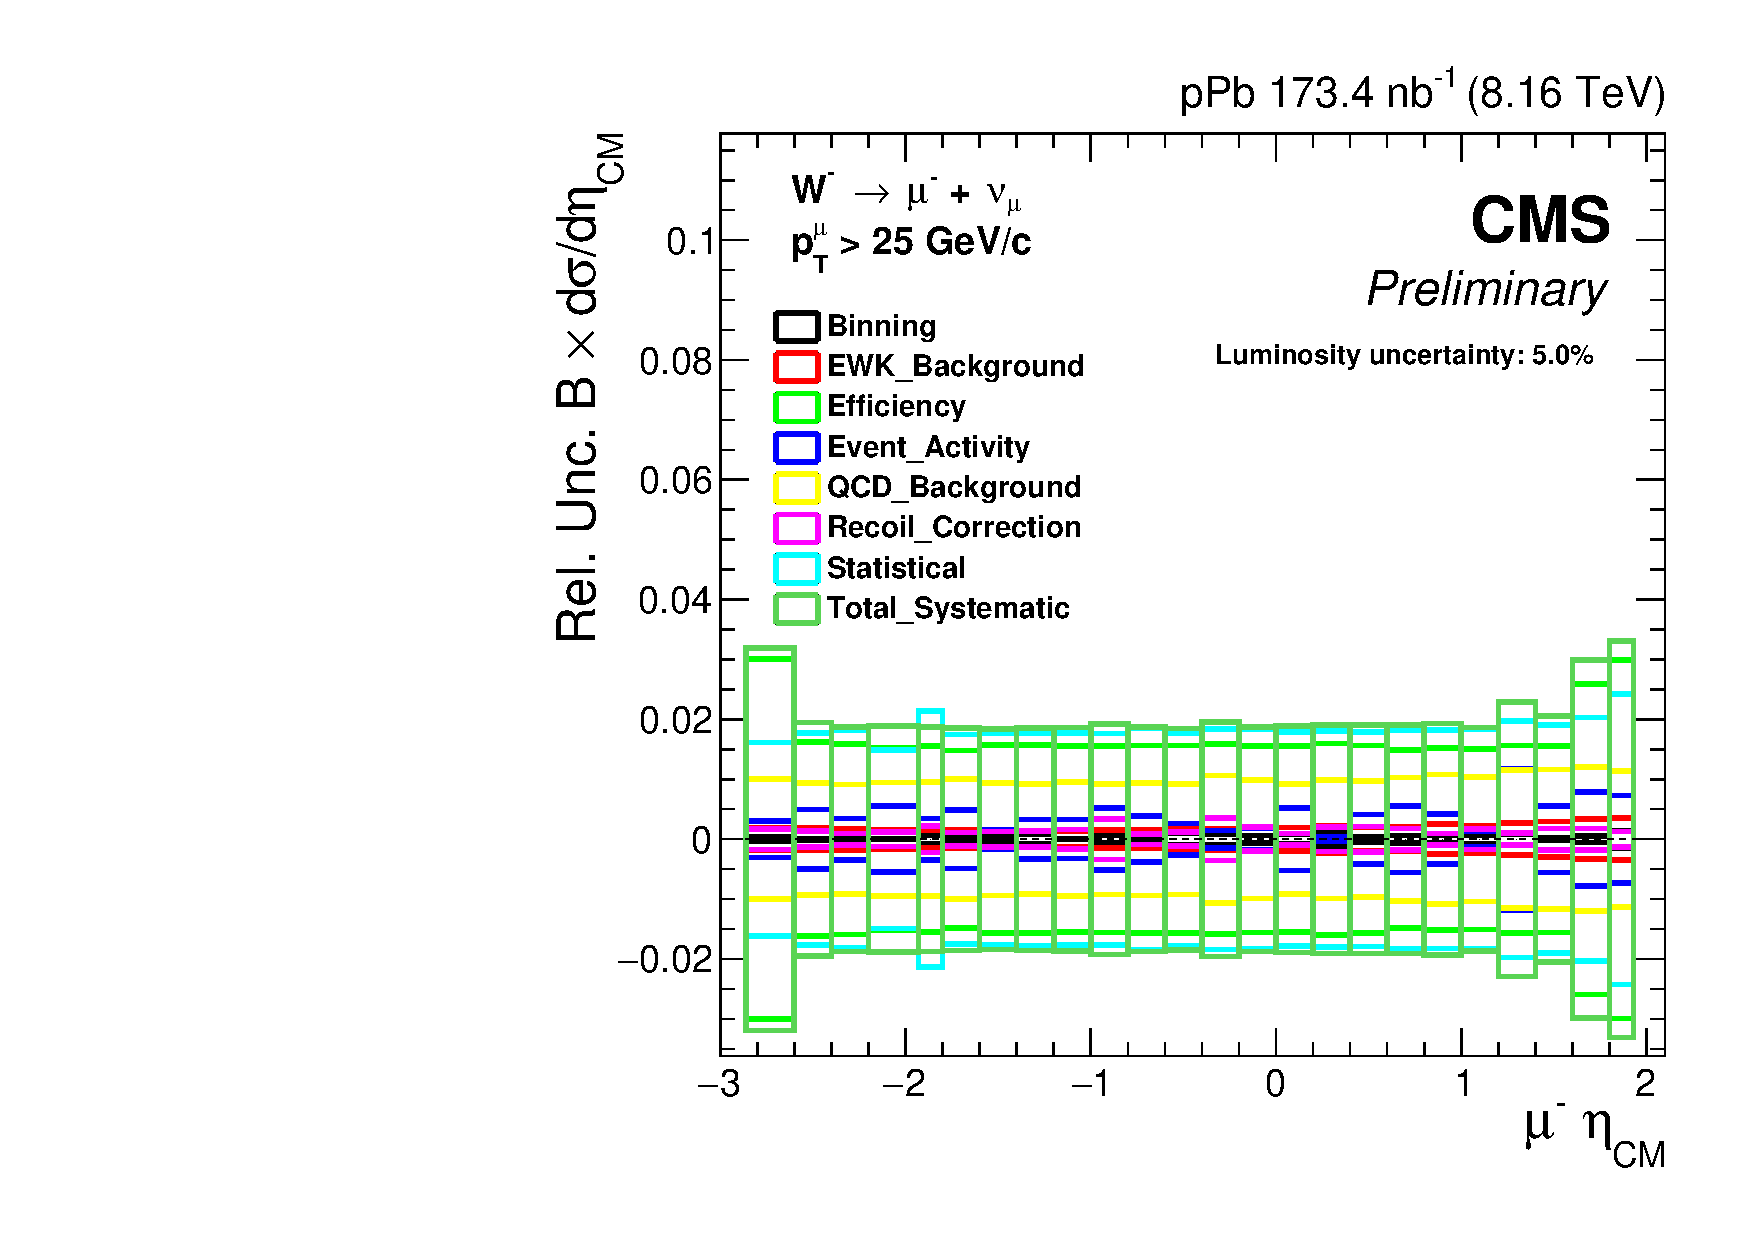
\includegraphics[width=0.30\textwidth]{Figures/WBoson/Analysis/Systematics/Combined/PA/Cross_Section/gr_WToMuMi_PA_Cross_Section_EffTnP.pdf}
  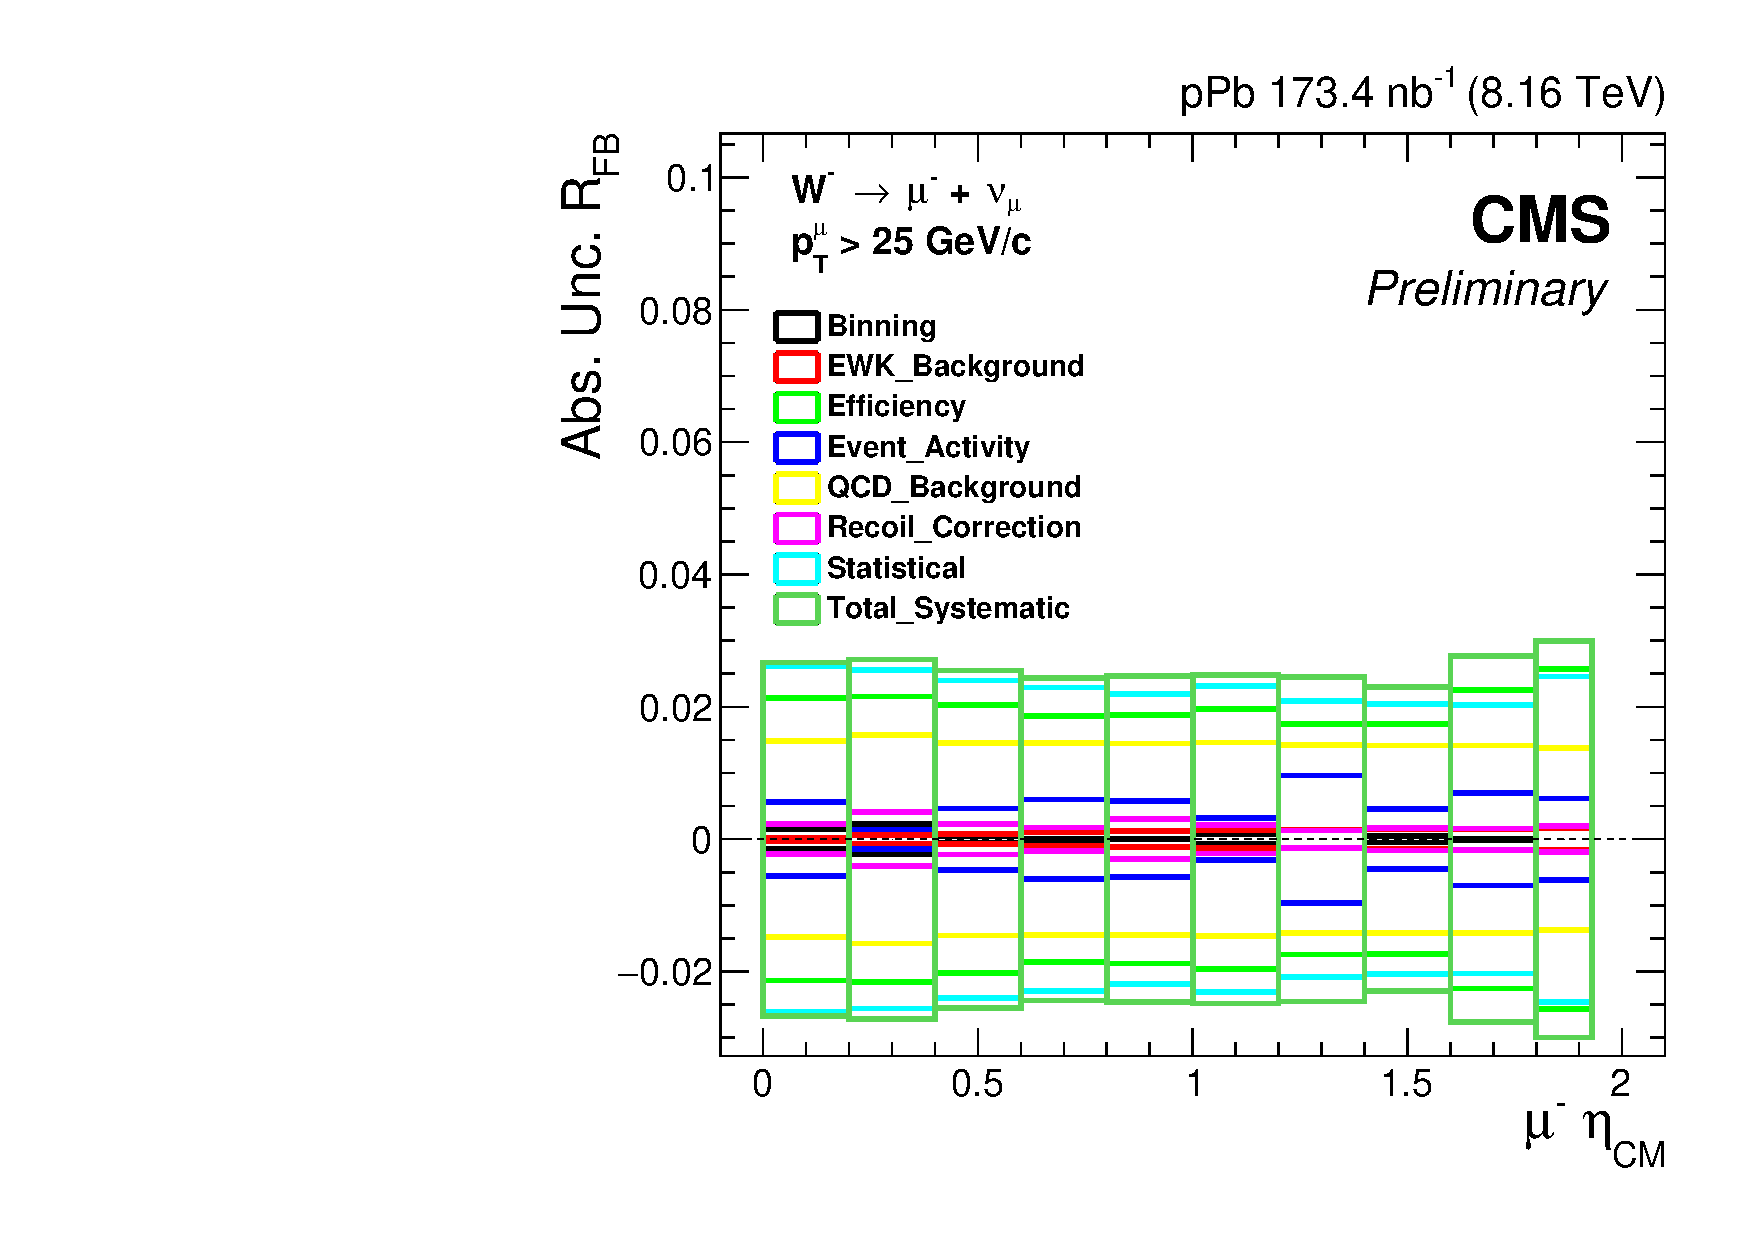
\includegraphics[width=0.30\textwidth]{Figures/WBoson/Analysis/Systematics/Combined/PA/ForwardBackward_Ratio/gr_WToMuMi_PA_ForwardBackward_Ratio_EffTnP.pdf}
  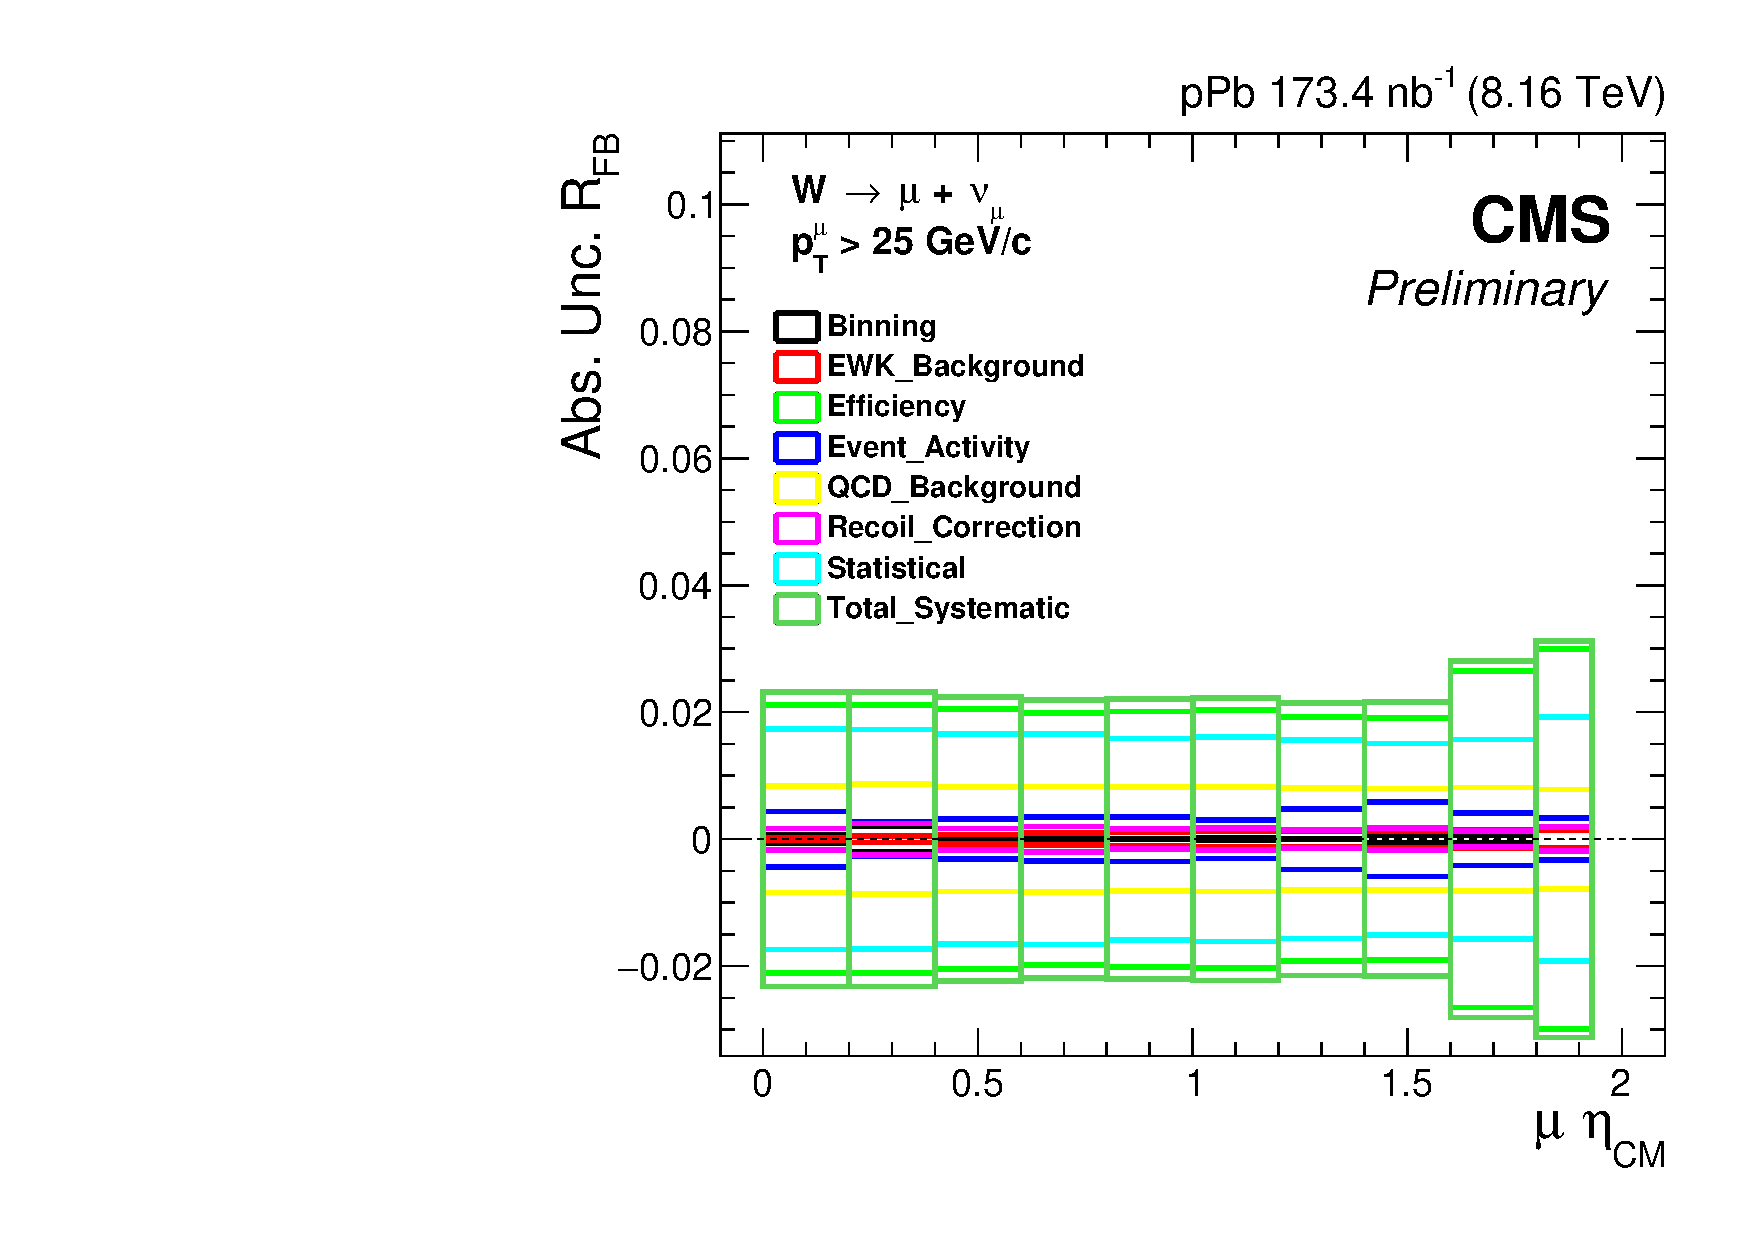
\includegraphics[width=0.30\textwidth]{Figures/WBoson/Analysis/Systematics/Combined/PA/ForwardBackward_Ratio/gr_WToMuInc_PA_ForwardBackward_Ratio_EffTnP.pdf}
%%
  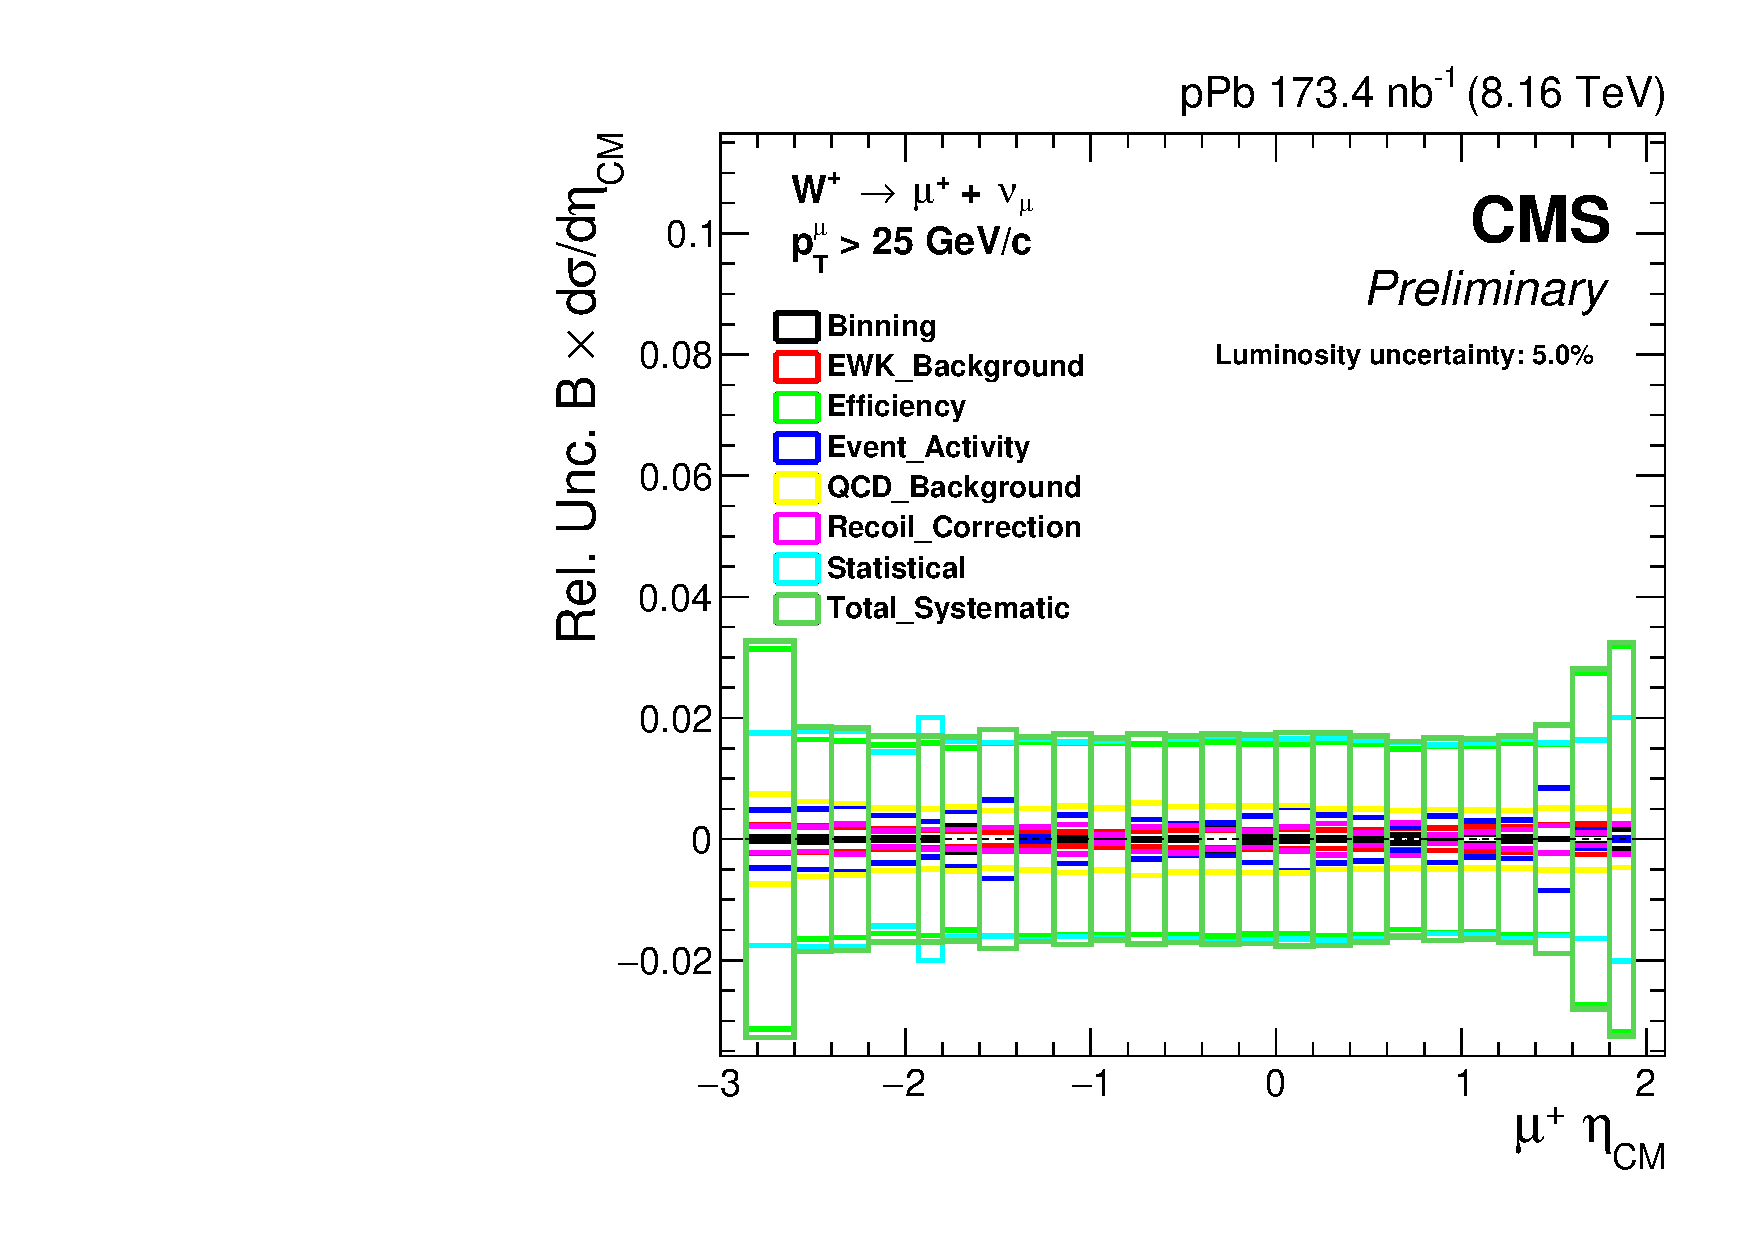
\includegraphics[width=0.30\textwidth]{Figures/WBoson/Analysis/Systematics/Combined/PA/Cross_Section/gr_WToMuPl_PA_Cross_Section_EffTnP.pdf}
  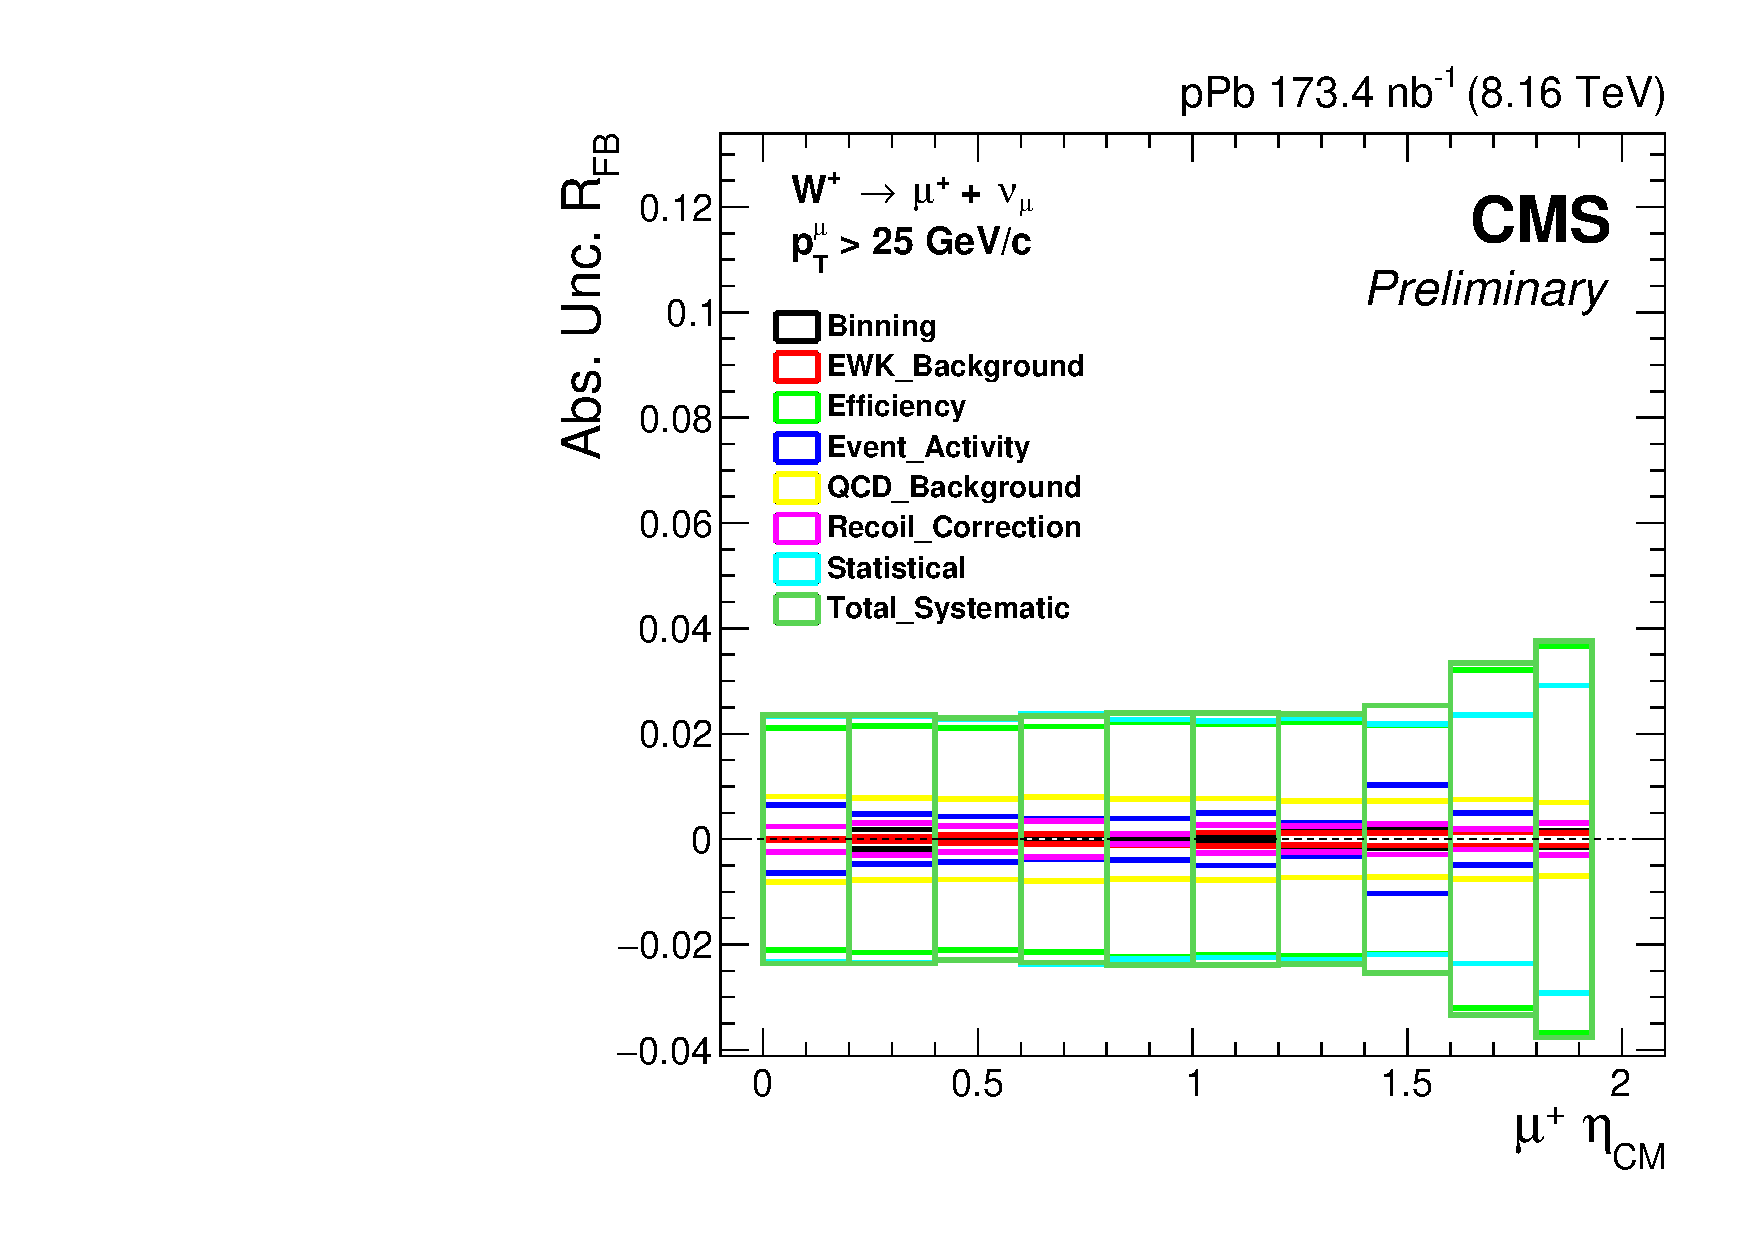
\includegraphics[width=0.30\textwidth]{Figures/WBoson/Analysis/Systematics/Combined/PA/ForwardBackward_Ratio/gr_WToMuPl_PA_ForwardBackward_Ratio_EffTnP.pdf}
  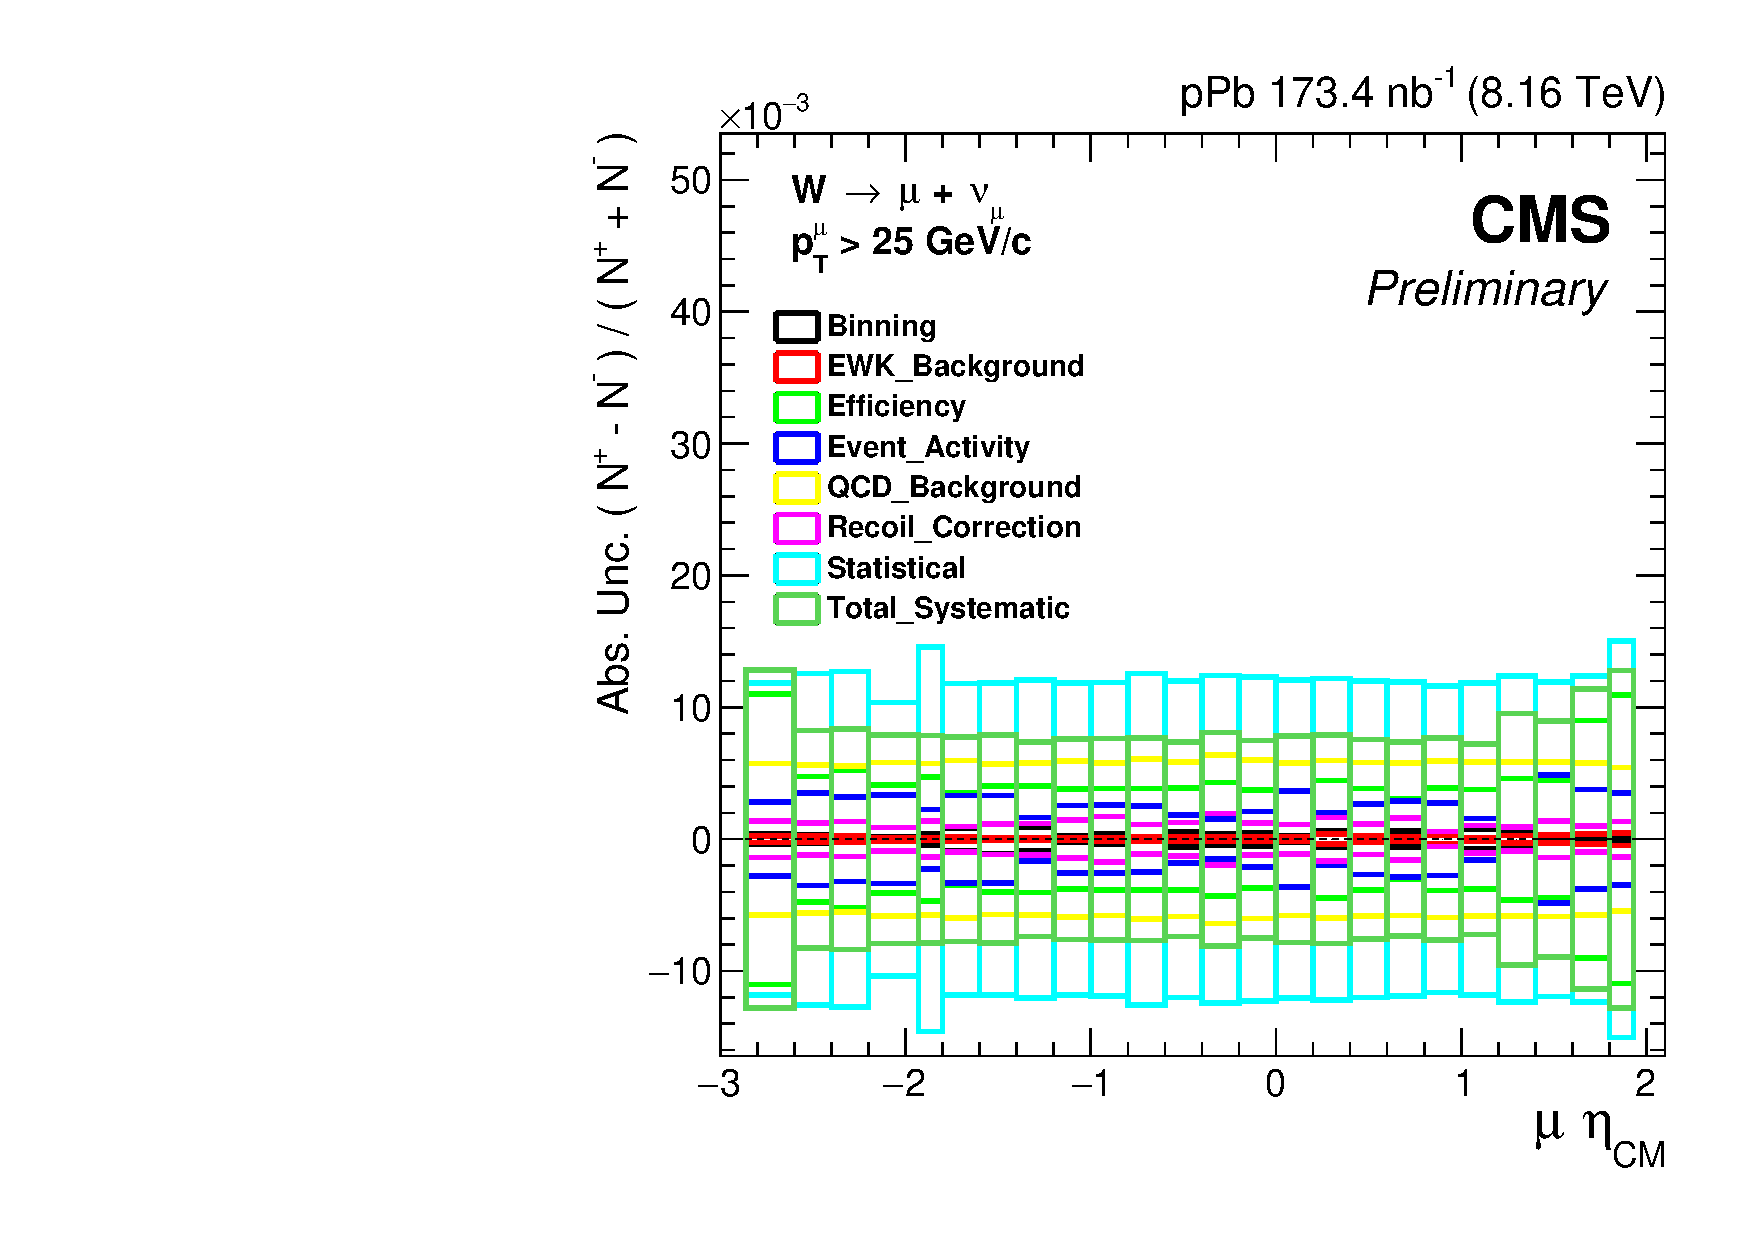
\includegraphics[width=0.30\textwidth]{Figures/WBoson/Analysis/Systematics/Combined/PA/Charge_Asymmetry/gr_WToMuInc_PA_Charge_Asymmetry_EffTnP.pdf}
 \end{center}
 \caption{Uncertainty corresponding to each category as function of the muon $\eta_{CM}$. The plots are divided as: \WToMuNuMi (top-left) and \WToMuNuPl (bottom-left) cross sections, $\W^{-}$ (top-middle) and $\W^{+}$ (bottom-middle) $R_{FB}$, and finally the \W $R_{FB}$ (top-right) and \W charge asymmetry (bottom-right). The uncertainties of the cross sections are relative while for the asymmetries are absolute. The global luminosity uncertainty of $\pm$5.0$\%$ is not included.}
 \label{fig:Summary_Systematics}
\end{figure}

%%------------------------------------------------------------%%
\subsection{Covariance matrix}\label{sec:WBoson_Systematics_CovarianceMatrix}

The covariance matrix of the systematic uncertainties is computed by combining all the bins of each observable to account for the bin-to-bin correlations. In the case of the $\W^{\pm}$ cross sections and the $\W^{\pm}$ forward-backward ratios, the matrix is made using 48 bins (24 pseudorapidity bins times 2 charge bins), while for the charge asymmetry and the charge-inclusive $R_{FB}$ only 24 bins are considered.

For a given (i,j) entry of the matrix, the covariance is calculated as the error in bin i times the error in bin j. If the uncertainty is uncorrelated, the off-diagonal elements are set to zero. The total covariance matrix is computed by summing the matrices of each uncertainty.

The total correlation matrix of each observable is derived from the total covariance matrix by using the following formula $corr(i,j) = cov(i,j)/(\sqrt{cov(i,i)*cov(j,j)})$. The corresponding correlation matrices are displayed in \fig{fig:CorrelationMatrix}. The black lines are used to distinguish the different bins of muon charge which are ordered in a given plot from top to bottom as: Minus-Minus , Minus-Plus, Plus-Minus and Plus-Plus.

\begin{figure}[!h]
 \begin{center}
  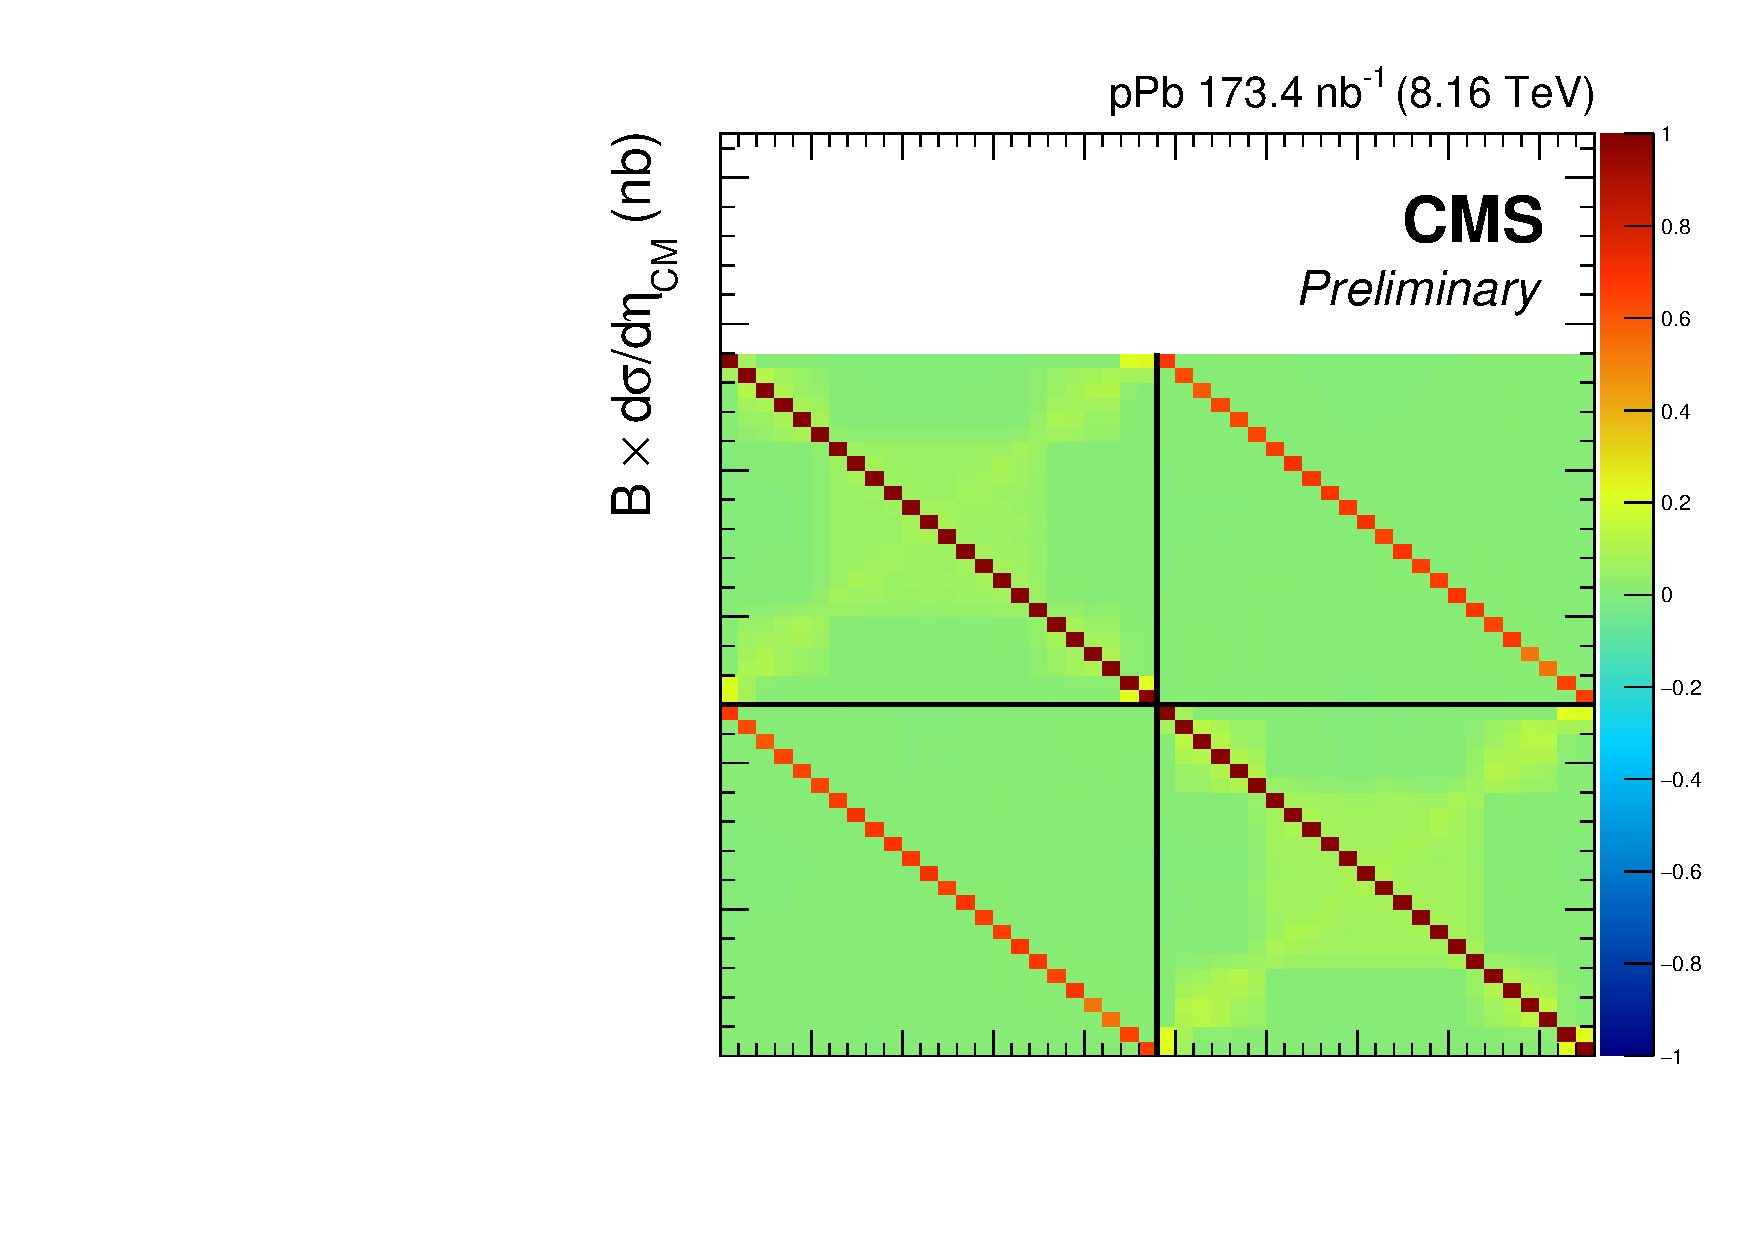
\includegraphics[width=0.40\textwidth]{Figures/WBoson/Analysis/CovarianceMatrix/PA/Cross_Section/covMatrix_WToMuPl_PA_Cross_Section_Total_Total.pdf}
  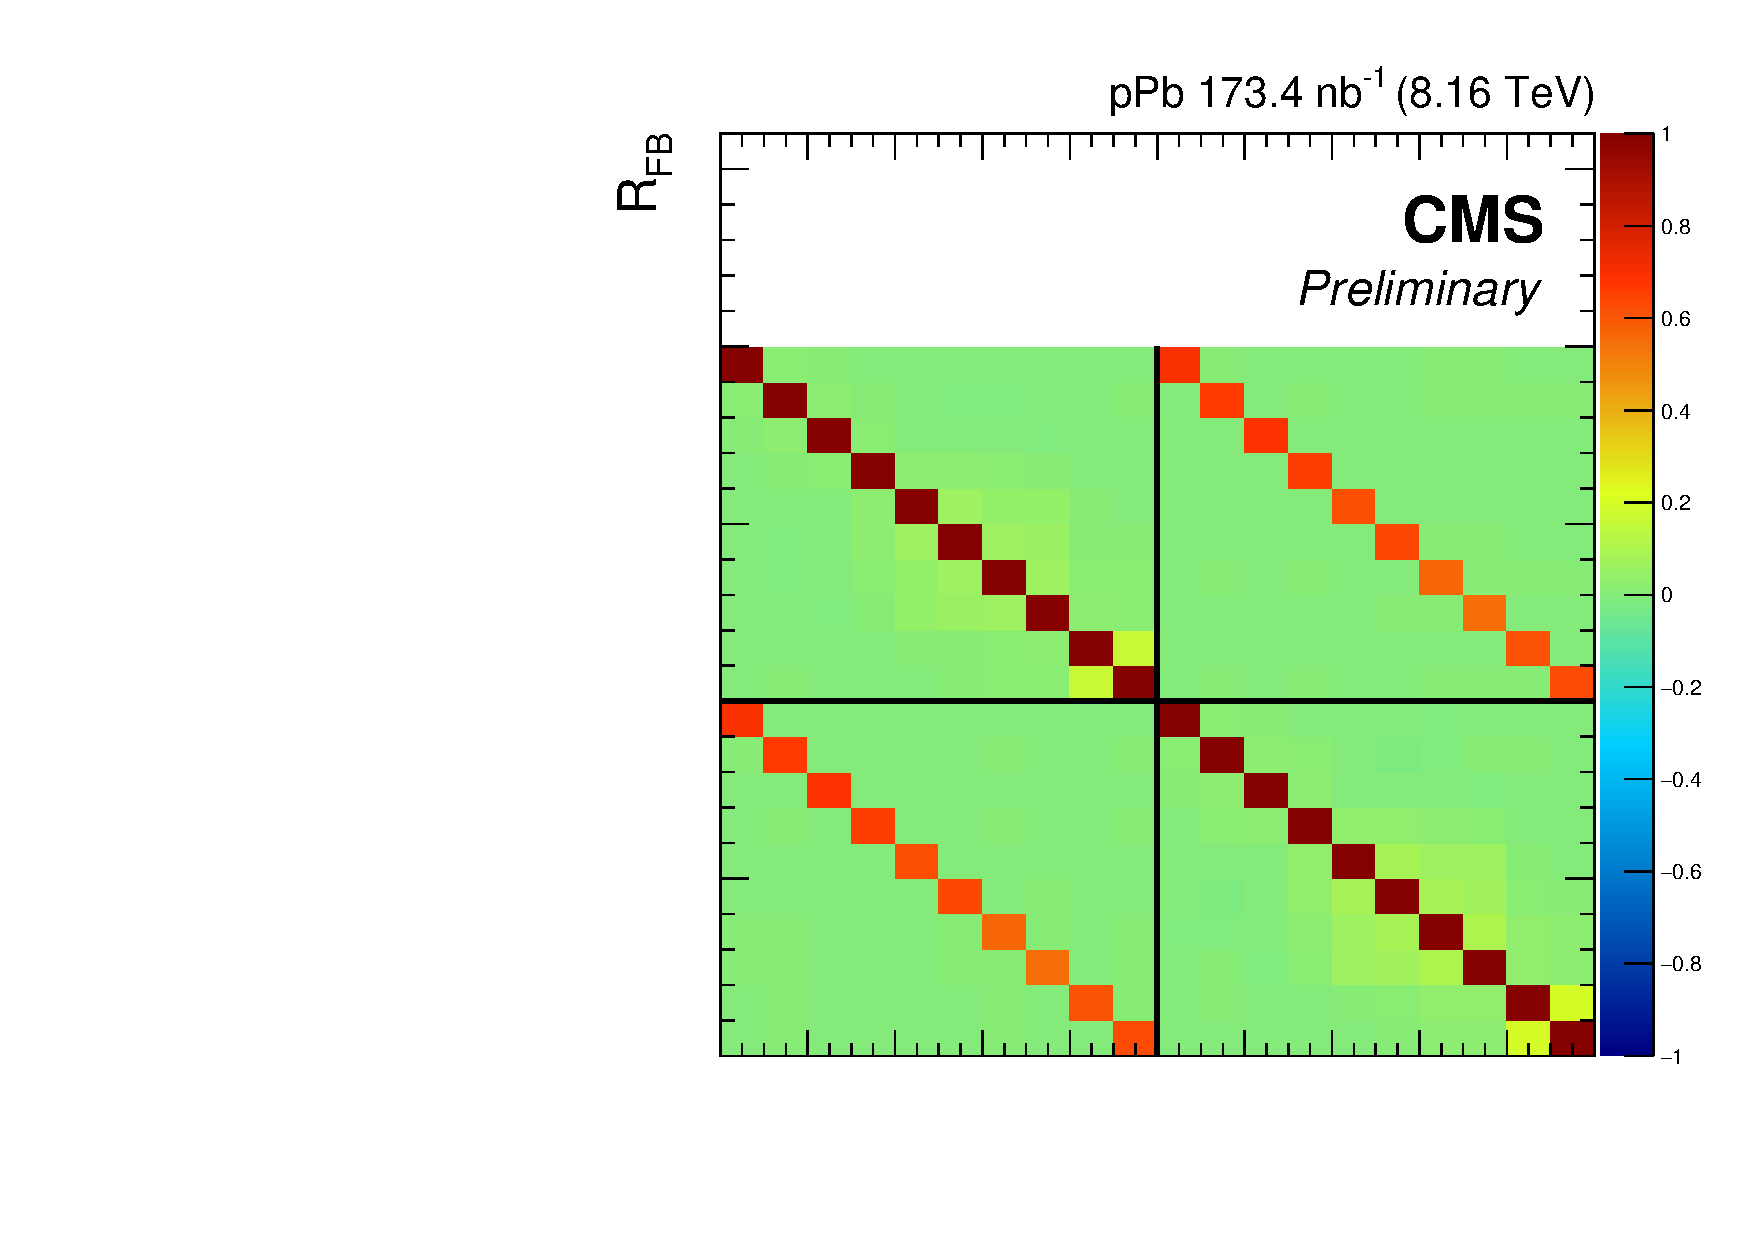
\includegraphics[width=0.40\textwidth]{Figures/WBoson/Analysis/CovarianceMatrix/PA/ForwardBackward_Ratio/covMatrix_WToMuPl_PA_ForwardBackward_Ratio_Total_Total.pdf}
%%
  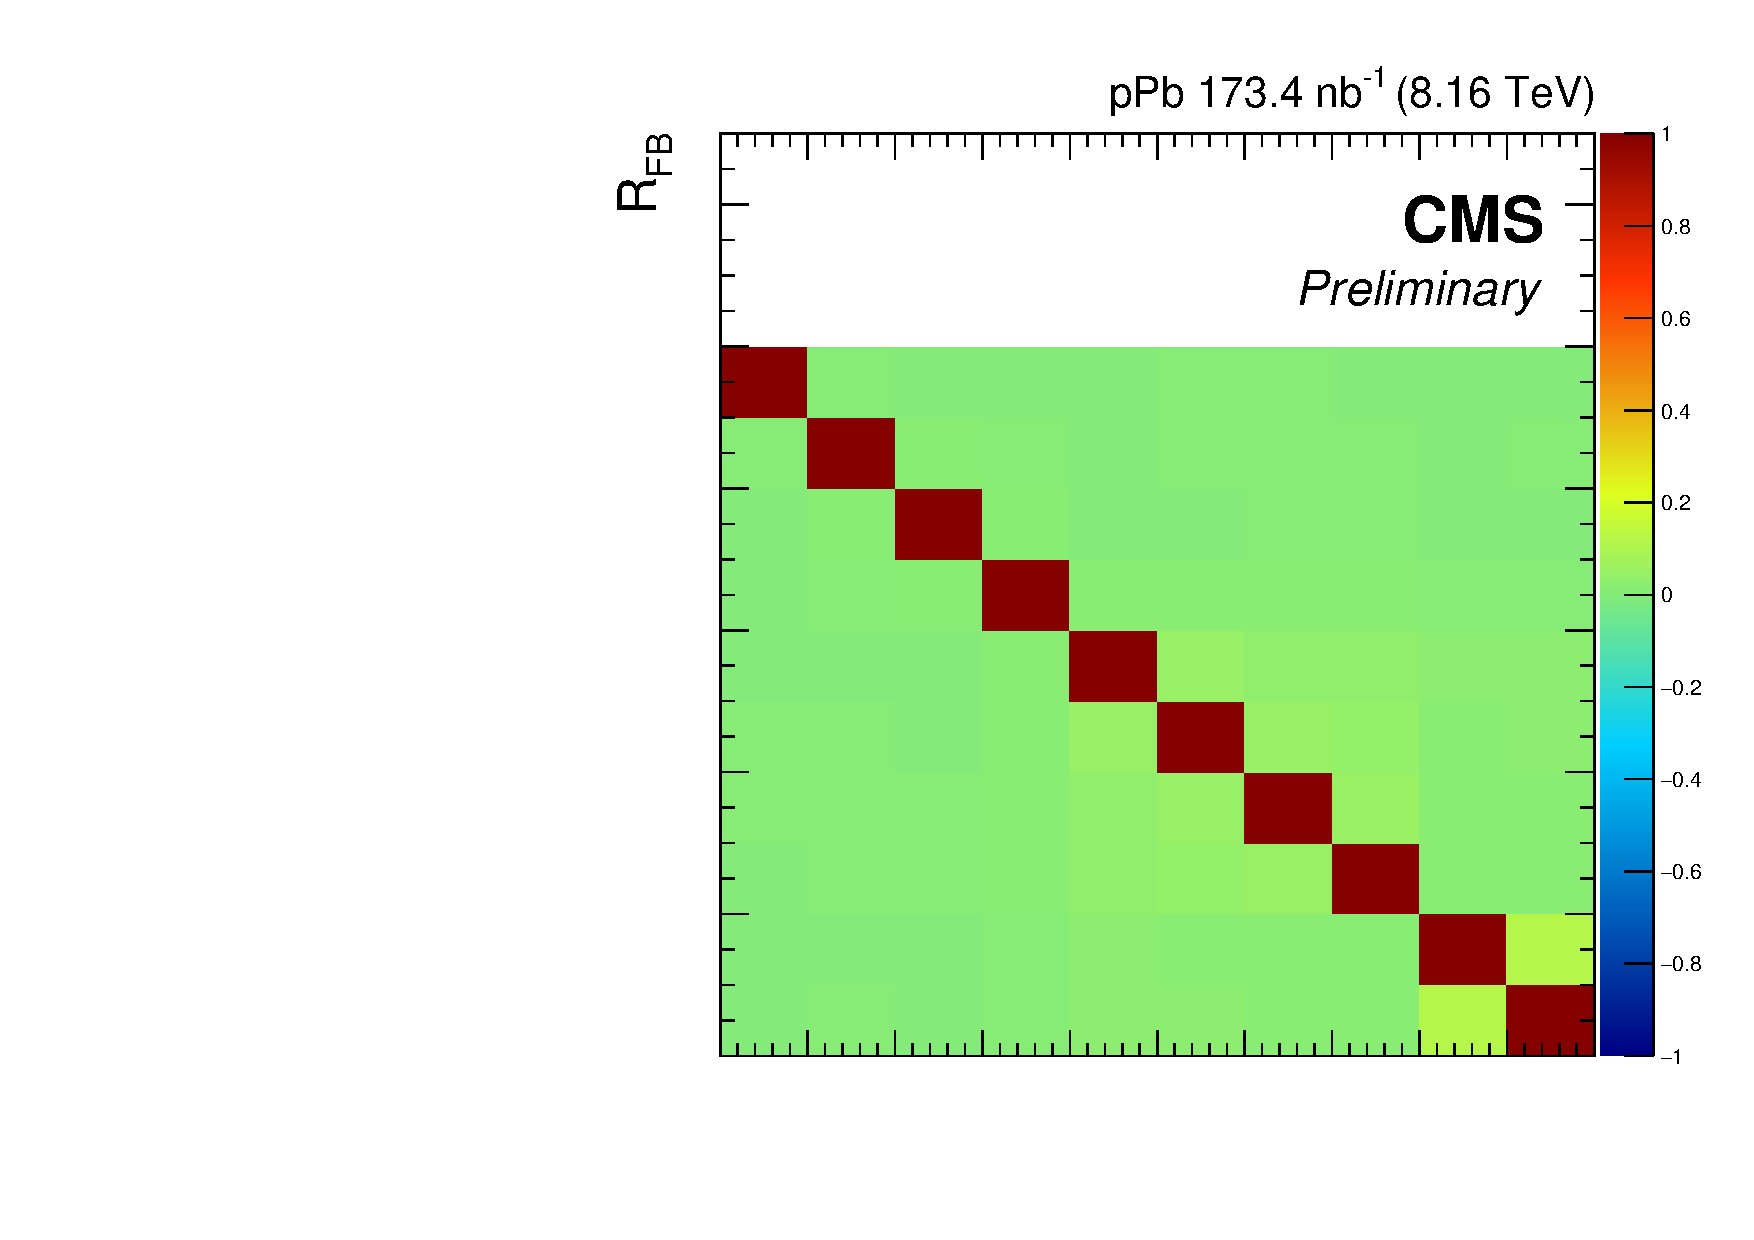
\includegraphics[width=0.40\textwidth]{Figures/WBoson/Analysis/CovarianceMatrix/PA/ForwardBackward_Ratio/covMatrix_WToMu_PA_ForwardBackward_Ratio_Total_Total.pdf}
  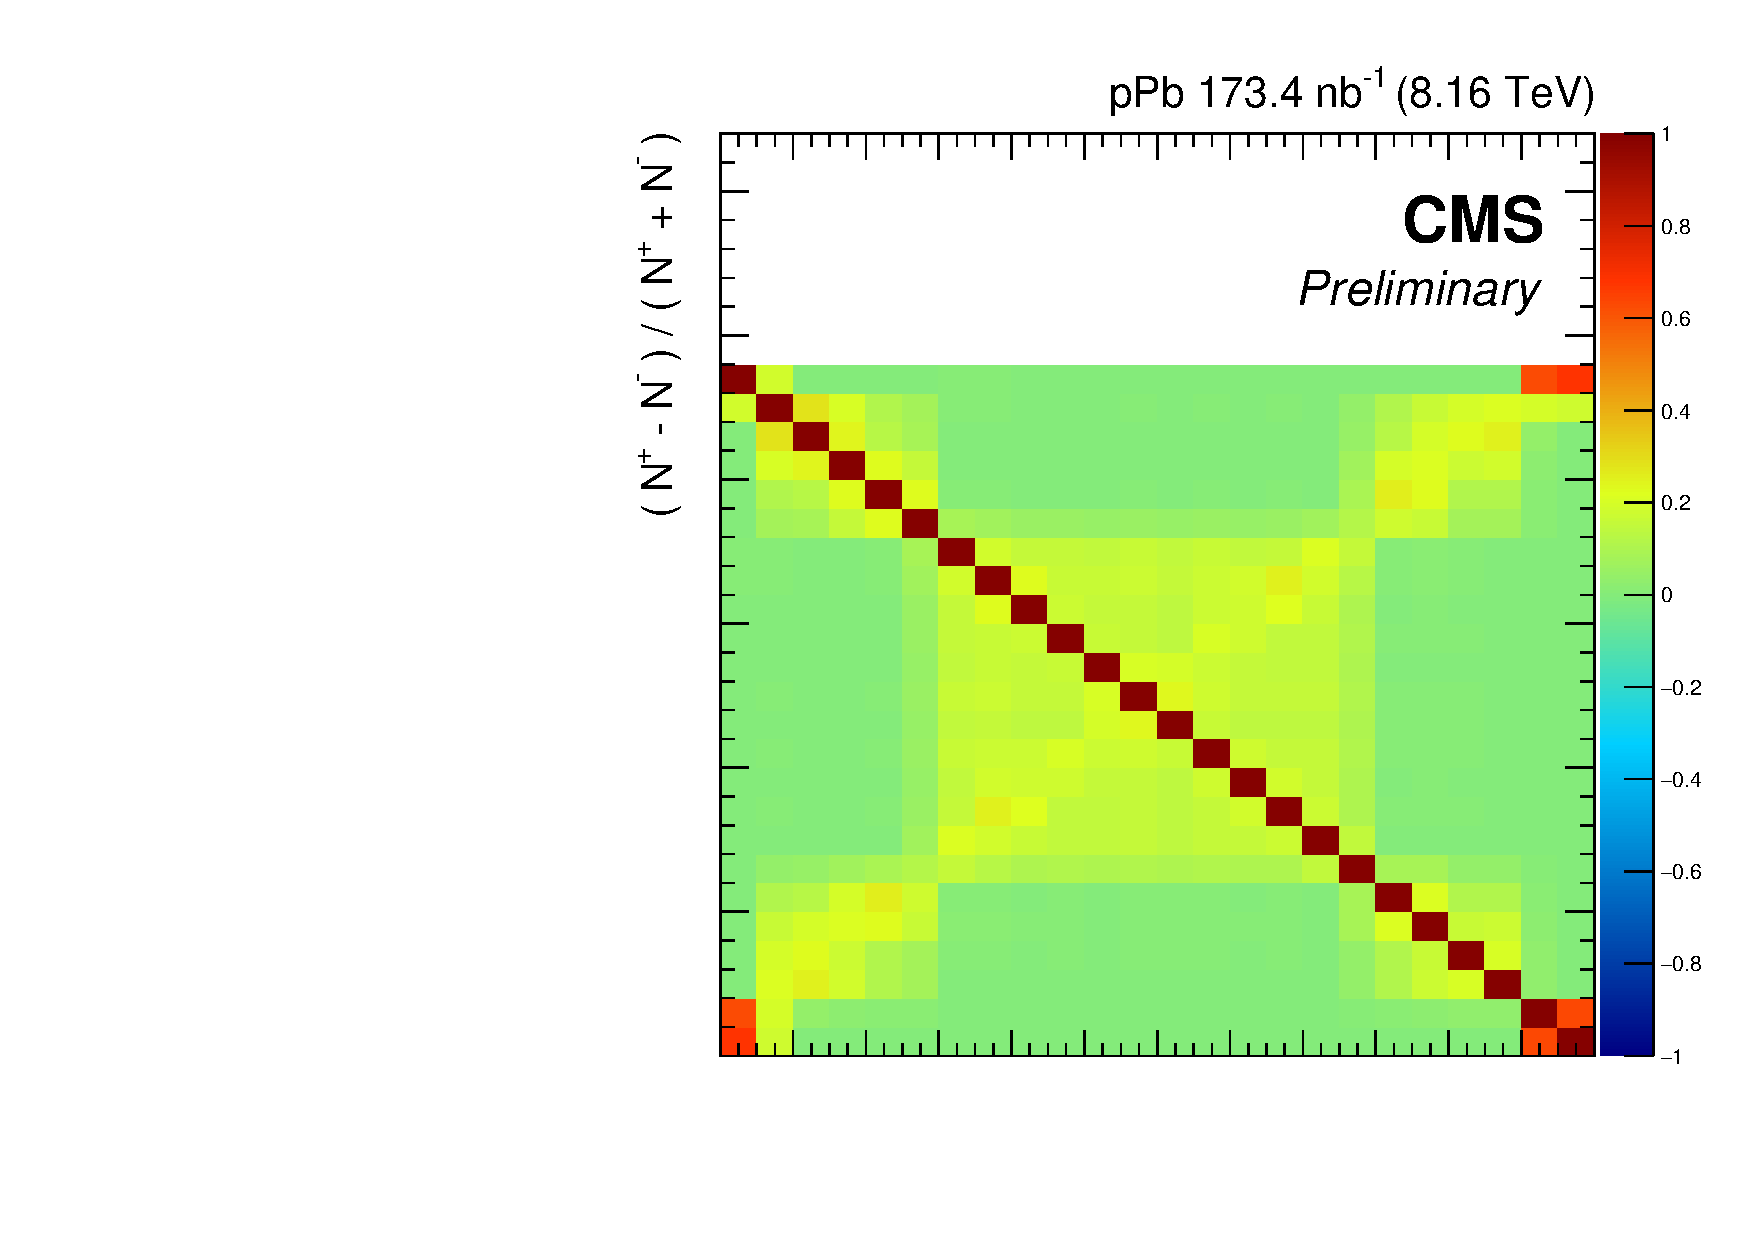
\includegraphics[width=0.40\textwidth]{Figures/WBoson/Analysis/CovarianceMatrix/PA/Charge_Asymmetry/covMatrix_WToMu_PA_Charge_Asymmetry_Total_Total.pdf}
 \end{center}
 \caption{Correlation matrix of the systematic uncertainties. The plots are divided as: $\W^{\pm}$ cross section (top-left) , $\W^{\pm}$ $R_{FB}$ (top-right) , charge-inclusive $R_{FB}$ (bottom-left) , and charge asymmetry (bottom-right). The lines in the top plots are used to separate the different muon charge bins.}
 \label{fig:CorrelationMatrix}
\end{figure}


% END OF SUBSECTION
